\documentclass[aspectratio=169]{beamer}

\usepackage{graphicx,fulda,german,float, tabto}

\setbeamertemplate{section in toc}[sections numbered]

% Title
\title[Cloud Computing]{Cloud Computing WiSe 19}
\subtitle{SciTub - Video On Demand on Microsoft Azure}
\author[Hildebrandt, Herche]{Benjamin Hildebrandt \\ Markus Herche}
\institute{Fachbereich Angewandte Informatik\\Hochschule Fulda -- University of Applied Sciences}

\begin{document}

\begingroup
\setbeamertemplate{background}[default]
\begin{frame}[plain]
  \titlepage
\end{frame}
\endgroup

\begin{frame}
  \frametitle{Inhaltsverzeichnis}
  \tableofcontents
\end{frame}

%%%%% Architektur Teil
% Kurzer Gesamtüberblick über die verwendete Architektur.
\section{Architektur}
\begin{frame}
  \frametitle{Architektur}
  \framesubtitle{Überblick}
  %Stichpunkte
  \begin{minipage}{.45\textwidth}
    \begin{itemize}
      \item Verwendung der \textbf{A}zure \textbf{M}edia \textbf{S}ervices
      \item Abwandlung der von Microsoft vorgeschlagenen Architektur
      \item Upload und Bereitstellung über einen entsprechenden Webservice
      \item Speicherung der Metadaten in einer Datenbank
      \item Erweiterbarkeit: CDN mit einfachen Schritten implementierbar
    \end{itemize}
  \end{minipage}
  %Abbildung
  \begin{minipage}{.5\textwidth}
    \begin{figure}[H]
      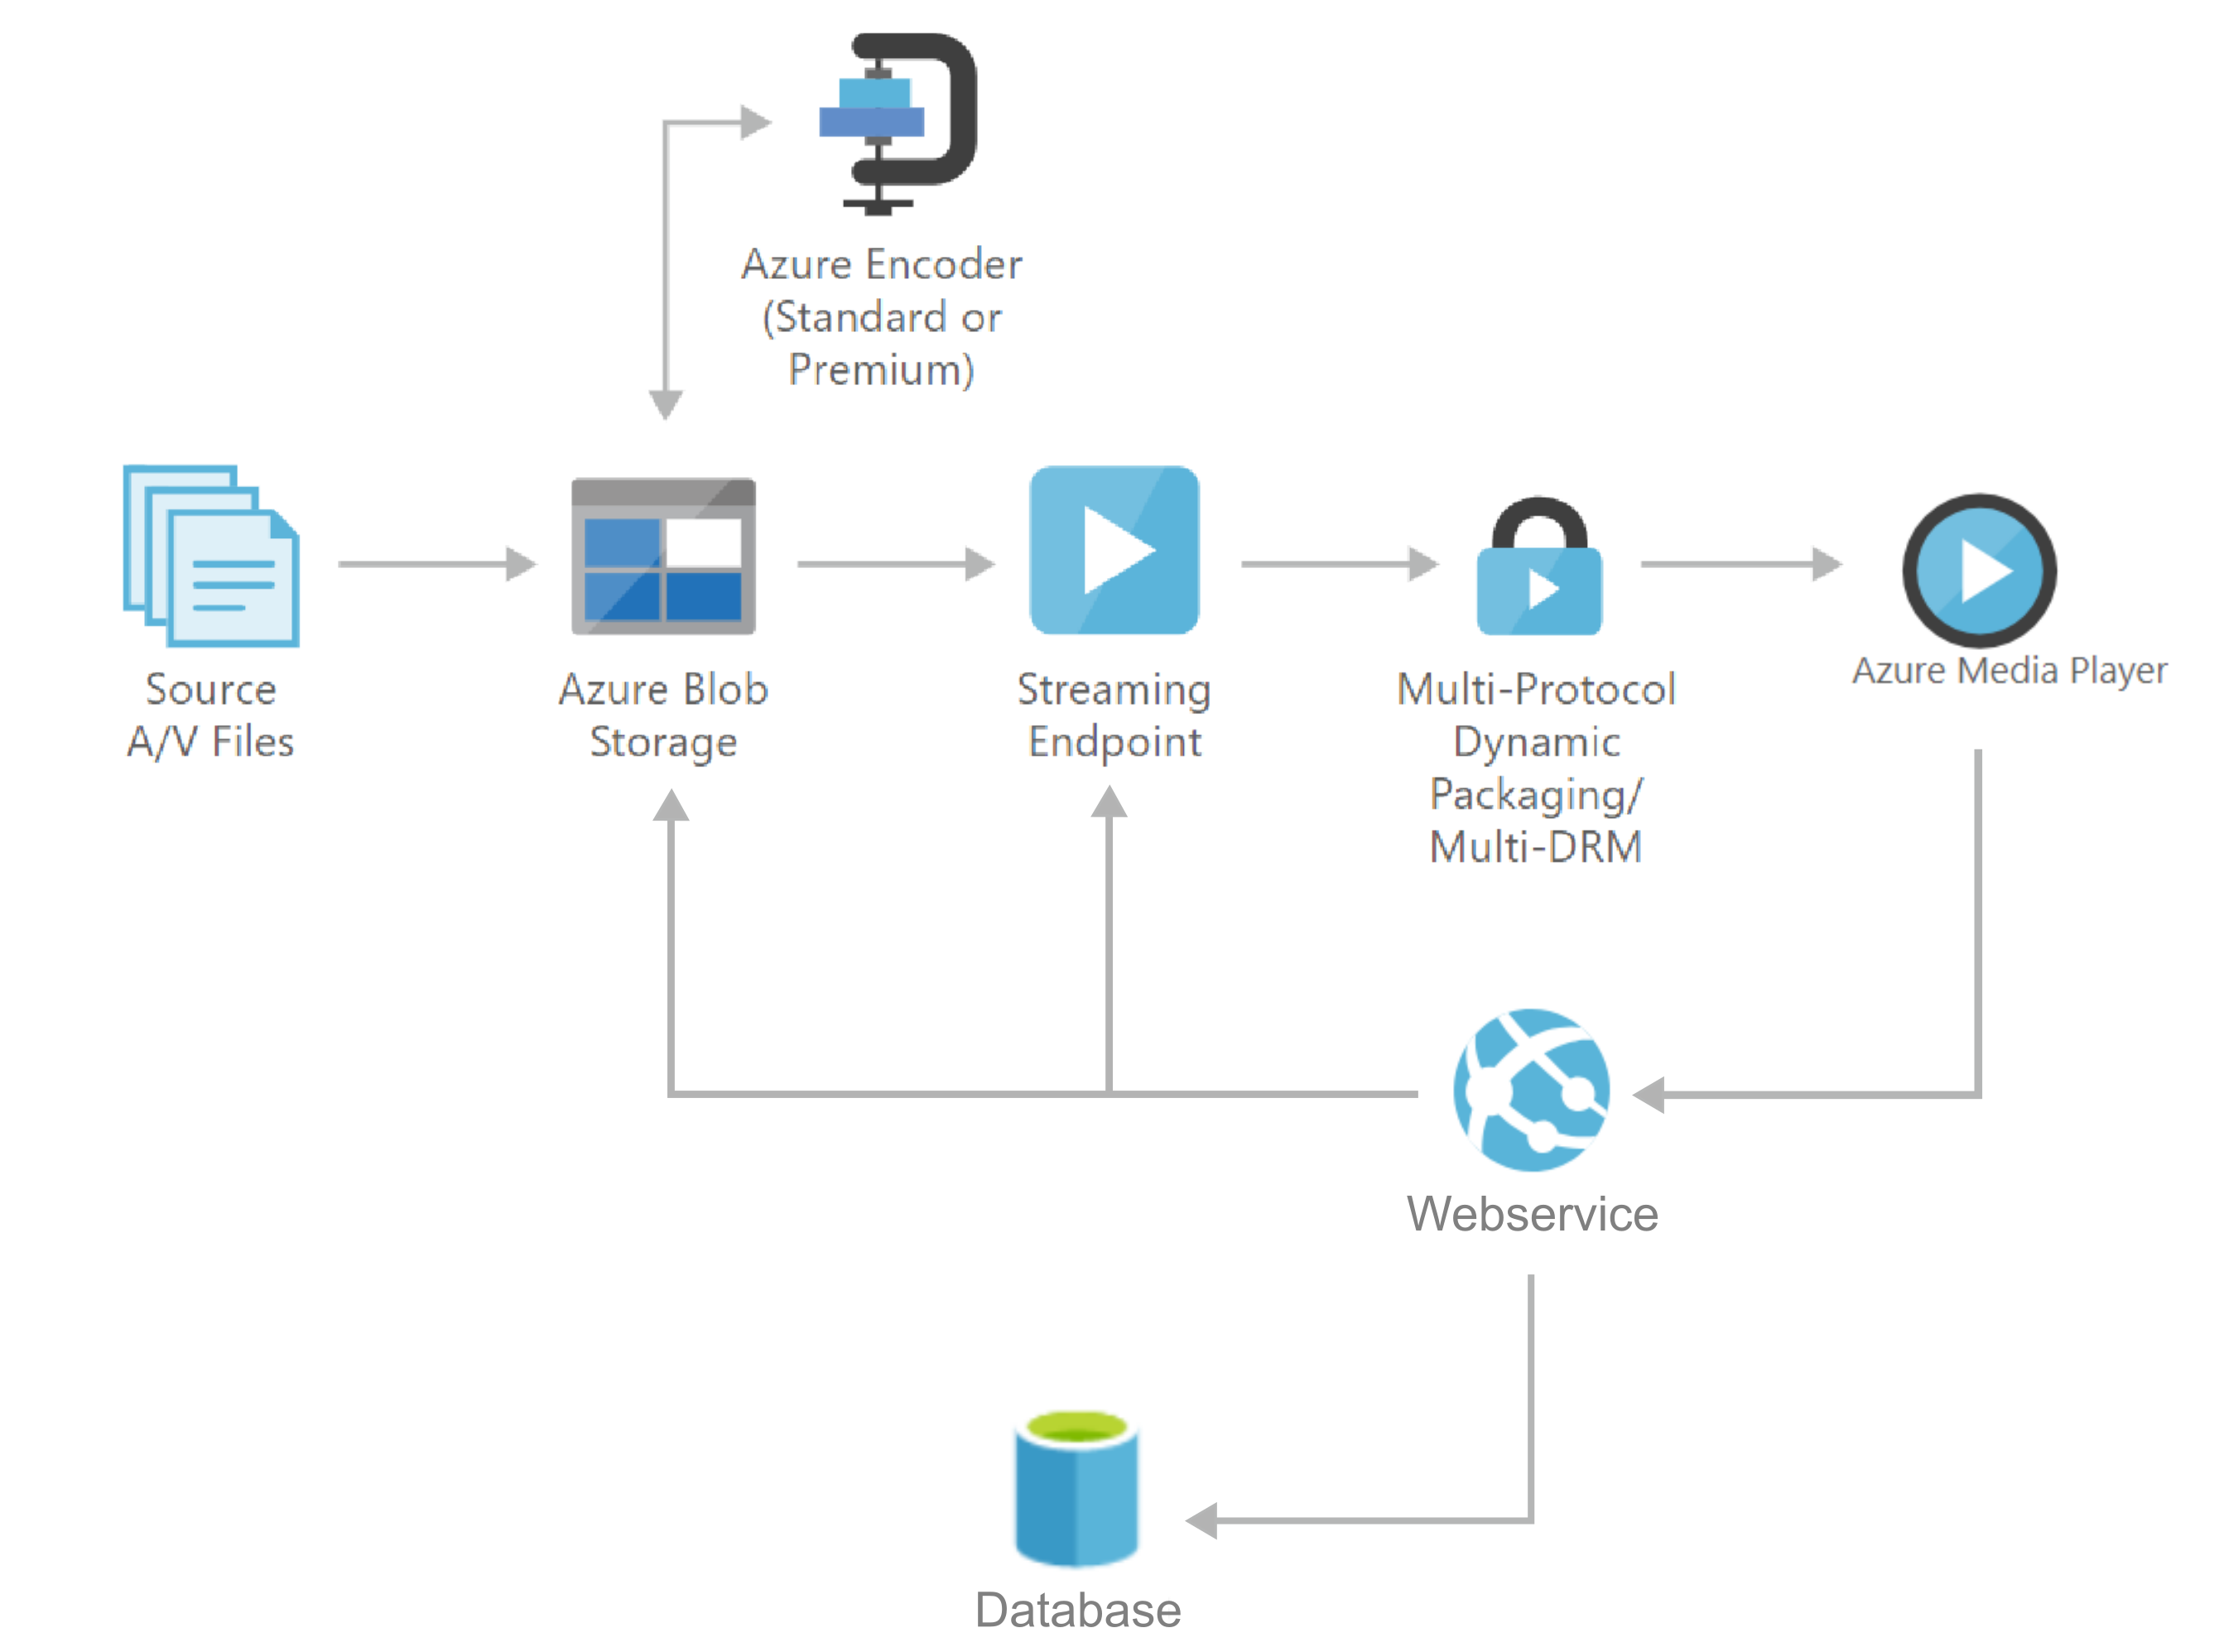
\includegraphics[height=130px]{img/architecture_new.png}
      \caption{SciTube Architektur}
      \label{fig:arch_new}
    \end{figure}
  \end{minipage}
\end{frame}

% Breakdown: Kurze Erläuterung der WICHTIGSTEN Teile der Architektur. Während der Vorstellung darauf eingehen, wie die entsprechenden Teile (potentiell) skalieren
\begin{frame}
  \frametitle{Architektur}
  \framesubtitle{Breakdown}
  \begin{itemize}
    \item \textbf{Azure Blob Storage:} Günstiger Speicherplatz für hochgeladene Files/Videos
    \item \textbf{Streaming Endpoint:} Stellt Inhalte zur weiteren Verteilung dar (an Client oder CDN)
    \item \textbf{Azure Media Encoder:} Codierung von Assets (Videos) für adaptives Streamen oder Smooth Streaming
    \item \textbf{Webservice:} Schnittstelle zwischen Azure und Client. Upload der Files werden hier verarbeitet und vorhandene Videos abgerufen.
    \item \textbf{Database:} Umfasst alle Metadaten der Files und (später) Nutzerdaten
  \end{itemize}
\end{frame}

%%%%% NIST-Kriterien
% Werden alle Kriterien erfüllt? Ja, die meisten schon durch die Nutzung von Azure
\section{NIST-Kriterien}
\begin{frame}
  \frametitle{NIST-Kriterien}
  \framesubtitle{Ist das eine Cloud-Anwendung?}
  \begin{itemize}
    \item \textbf{On-Demand Self Service:} UI durch Dashboard und APIs
    \item \textbf{Broad Network Access:} Übertragung von ``gewöhnlichen'' Datenarten
    \item \textbf{Resource Pooling:} Wir kennen nicht den Aufbau von MS-Datencentern...
    \item \textbf{Rapid Elasticity:} Automatische Skalierung (Grenzwerte nicht untersucht)
    \item \textbf{Measured Services:} Abrechnung pro Nutzungstakt, tabellarisch einsehbar
    \end{itemize}
\end{frame}

\begin{frame}
  \frametitle{NIST-Kriterien}
  \framesubtitle{Ist das eine Cloud-Anwendung?}
%  \begin{tabbing}    %https://tex.stackexchange.com/questions/14038/tabbing-inside-itemize-or-itemize-inside-tabbing
  \begin{itemize}
    \item \textbf{On-Demand Self Service}\tabto{6cm}\checkmark 
    %\hspace{1em} \= \checkmark  1 st line, set tabbing
    \item \textbf{Broad Network Access}\tabto{6cm}  \checkmark   %\>
    \item \textbf{Resource Pooling}\tabto{6cm} \checkmark
    \item \textbf{Rapid Elasticity}\tabto{6cm}\checkmark
    \item \textbf{Measured Services}\tabto{6cm}\checkmark
  \end{itemize}
%  \end{tabbing}
\end{frame}

%%%%% Funktionsweise
% Vorstellung des Videostreamings. 
\section{Funktionsweise}
\begin{frame}
  \frametitle{Funktionsweise}
  \framesubtitle{Streamen eines Videos}
  \begin{enumerate}
    \item Aufruf der \texttt{Webservice} Schnittstelle für alle Videos durch den Benutzer
    \item \texttt{Webservice} fragt alle Videodaten aus der Datenbank (inkl. des Azure Streaming Links) ab
    \item \texttt{Webservice} gibt Metadaten an Client weiter
    \item Aufruf des Videos durch Benutzer 
    \item Zugriff des Azure Media Players auf den \texttt{Streaming Endpoint}
  \end{enumerate}
\end{frame}

\begin{frame}
  \frametitle{Funktionsweise}
  \framesubtitle{Upload eines Videos}
  \begin{enumerate}
    \item Upload der Videodatei  von Client an \texttt{Webservice}
    \item Der \texttt{Webservice} ruft die Schnittstelle von \textbf{AMS} auf:
    \begin{enumerate}
      \item Erstellen eines Assets und Upload des Videos
      \item Anlegen und Anwendung eines Encoding-Jobs für das Asset
      \item Speicherung der Metadaten nach Beendigung des Jobs in der Datenbank
    \end{enumerate}
    \item Löschung der Datei vom Webservice
  \end{enumerate}
\end{frame}

%%%%% Demo Teil
\section{Script und Live Demo}
\begin{frame}
  \frametitle{Live Demo}
  \centering
  \begin{figure}[H]
    
\includegraphics[height=50px, width=75px]{img/live.png}
    \label{fig:live}
  \end{figure}
\end{frame}

\end{document}
  